% !TeX encoding = UTF-8
% !TeX spellcheck = en_US
% !TeX TXS-program:bibliography = biber -l zh__pinyin --output-safechars %
%% !TeX TS-program = xelatex

\documentclass[a4paper,10pt]{article}

\newcommand{\hwNumber}{5}

% to be `\input` in subfolders,
% ... therefore the path should be relative to subfolders.

\usepackage[UTF8
	,heading=false
	,scheme=plain % English Document
]{ctex}
\usepackage{indentfirst}

\input{../.modules/basics/macros.tex}
\input{../.modules/preamble_base.tex}
\input{../.modules/preamble_notes.tex}

\newcommand{\legacyReference}{{
	\clearpage\par
	\quad\clearpage
	\renewcommand{\midquote}{\textbf{PAST WORK, AS TEMPLATE}}
	\newparagraph
}}

% Settings
\counterwithout{equation}{section}
\mathtoolsset{showonlyrefs=false}
%\DeclareTextFontCommand{\textbf}{\sffamily}
\renewcommand{\midquote}{\quad}
\resizegathersetup{equations=false}

% Spacing
\geometry{footnotesep=2\baselineskip} % pre footnote split
\setlength{\parskip}{.5\baselineskip}
\renewcommand{\baselinestretch}{1.15}

%Title
	\posttitle{
		\hfill\Large\ccbyncsajp
		\par\end{flushleft}%
		\vspace*{-.7ex}\hrule%
	}
	\preauthor{\vspace{-1.5ex}%
		\flushleft\itshape%
	}
	\postauthor{\hfill}
	\predate{\noindent\ttfamily Compiled @ }
	\postdate{\vspace{.5ex}}

	\title{Finite Temperature Field Theory \textnumero\hwNumber}
	\author{\signature Bryan}
	\date{\today}

% List
	\setlist*{
		listparindent=\parindent
		,labelindent=\parindent
		,parsep=\parskip
		,itemsep=1.2\parskip
	}
	\setlist*[enumerate,1]{
		align=left
		,label=\fbox{\textbf{\arabic*}}
		,itemsep=.5\baselineskip
	}

\input{../.modules/basics/biblatex.tex}

%%% ID: sensitive, do NOT publish!
\InputIfFileExists{../id.tex}{}{}

\begin{document}
\maketitle
\pagestyle{headings}
\pagenumbering{arabic}
\thispagestyle{empty}

\vspace*{-1.5\baselineskip}

\subsection*{Correlations of Pauli Spinor Fields}
	The Lagrangian of a nonrelativistic free particle is given by:
	\begin{equation}
		\mcal{L}
		= \bar{\psi} \pqty{
				i\pdv{t} + \frac{\laplacian}{2m}
			} \psi
	\end{equation}
	The Euclidean action is then given by:
	\begin{equation}
		(-S) = \int \dd[4]{x}
			\mcal{L}_{t = -i\tau}
		= -\int \dd[4]{x}
			\bar{\psi} \pqty{
				\pdv{\tau} - \frac{\laplacian}{2m}
			} \psi
		= -\beta H
	\end{equation}
	
	Note that we have $
		N = \int \dd[3]{\vb{x}} \bar{\psi} \psi
		= \int \dd[3]{\vb{x}} n
	$ as a conserved charge, therefore it is natural to include $N$ in the partition function:
	\begin{equation}
		Z = \Tr e^{-\beta \pqty{H - \mu N}}
		= \int \DD\bar{\psi}\, \DD\psi\,
			\exp \int \dd[4]{x}
				\Bqty{
					- \bar{\psi} \pqty{
						\pdv{\tau} - \frac{\laplacian}{2m}
					} \psi
					+ \mu n
				}
	\end{equation}
	For a spin-$\frac{1}{2}$ free fermion, $\psi$ is given a 2-component Pauli spinor: $
		\psi \sim (\psi_+, \psi_-)
	$, and $\bar{\psi} = \psi^\dagger$ is the conjugate transpose of $\psi$. Relevant observables in the Heisenberg picture are then given by:
	\begin{gather}
		n = \psi^\dagger \psi,\quad
		\tilde{n} = n - \ave{n},\quad
		s_i = \psi^\dagger \sigma_i \psi,
	\\
		D_n = \ave[\Big]{
				\mcal{T}_\tau\,
					\tilde{n}(x)\,
					\tilde{n}(x')
			},\quad
		D_{ij} = \ave[\Big]{
				\mcal{T}_\tau\,
					s_i(x)\,
					s_j(x')
			}
	\end{gather}
	
	To compute the \textbf{density correlation} $D_n$, define the generating functional:
	\begin{equation}
		Z[j]
		= \int \DD\bar{\psi}\, \DD\psi\,
			\exp \int \dd[4]{x}
				\Bqty{
					- \bar{\psi} \pqty{
						\pdv{\tau} - \frac{\laplacian}{2m}
					} \psi
					+ \mu n(x)
					+ j(x)\,n(x)
				}
	\label{eq:generating_functional}
	\end{equation}
	To remove the non-zero $\ave{n}$, consider:
	\begin{gather}
		W[j] = \ln Z[j],\quad
		D_n = \ave[\Big]{
				\mcal{T}_\tau\,
					\tilde{n}(x)\,
					\tilde{n}(x')
			}
		= \eval{
				\frac{\var[2]{W[j]}}{
					\var{j(x)} \var{j(x')}
				}
			}_{j=0}\!\!
		= \eval{
				\frac{\var[2]{W^{(2)}[j]}}{
					\var{j(x)} \var{j(x')}
				}
			}_{j=0}
	\\[1ex]
		W^{(2)}
		\sim \order{j^2}
%		= \frac{\beta V}{2} \sum_q
%			j_q^\dagger\, D_n(q)\, j_q
	\end{gather}
	
	For free theory, $W^{(2)}$ can be computed explicitly by mode expansions:
	\begin{gather}
		\psi
		= \frac{1}{\sqrt{V}}
			\sum_k e^{ik\cdot x} \psi_k,\quad
		j
		= \sum_q e^{-iq\cdot x} j_q,\quad
		\sum_k e^{ik\cdot x}
		= V \int \frac{\dd[3]{\vb{k}}}{(2\pi)^3}\,
				e^{i\vb{k}\cdot\vb{x}}
			\sum_{n\in\mbb{Z}} e^{i\omega_n \tau}
%	\\
%		W^{(2)}
%		= \frac{\beta V}{2} \sum_q
%			j_q^\dagger\, D_n(q)\, j_q
	\end{gather}
	\begin{equation}
	\begin{aligned}
		Z[j]
		&= \int \DD\bar{\psi}\, \DD\psi\,
			\exp \int \dd[4]{x}
				\Bqty{
					- \bar{\psi}\, \pqty{
						\pdv{\tau}
						- \frac{\laplacian}{2m}
						- \mu - j(x)
					} \psi
				} \\
		&= \int \DD\bar{\psi}\, \DD\psi\,
			\exp \Bqty{
					- \beta \sum_{k,k'}
					\bar{\psi}_k\, \pqty\bigg{
						\pqty{
							i\omega
							+ \tfrac{\vb{k}^2}{2m}
							- \mu
						}\,\delta_{k,k'}
						- j_{k-k'}
					} \psi_{k'}
				} \\
		&\sim \Bqty\Big{\,
				\det_{k,k',\bullet} \pqty{
					\beta D_0^{-1}(k)
						\,\delta_{k,k'}
					- \beta j_{k-k'}
				}
			}^{-1},\quad
		D_0^{-1}(k)
		= i\omega
			+ \tfrac{\vb{k}^2}{2m}
			- \mu,\\
		&= \Bqty\Big{\,
				\det_{k,k'} \pqty{
					\beta D_0^{-1}(k)
						\,\delta_{k,k'}
					- \beta j_{k-k'}
				}
			}^{-2}
	\end{aligned}
	\end{equation}
	Note that the determinant should go over the implicit spinor indices as well, which results in a power of 2 in the final expression. 
	
	We can then compute $W[j]$ using Jacobi's formula:
	\begin{equation}
	\begin{aligned}
		W[j] = \ln Z[j]
		&= -2\ln \det_{k,k'} \pqty{
				\beta D_0^{-1}(k)\,\delta_{k,k'}
				- \beta j_{k-k'}
			} \\
		&= -2\operatorname*{Tr}\limits_{\,k,k'}
			\ln \pqty{
				\beta D_0^{-1}(k)\,\delta_{k,k'}
				- \beta j_{k-k'}
			} \\
		&= -2\operatorname*{Tr}\limits_{\,k,k'}
			\Bqty\Big{
				\delta_{k,k'} \ln \pqty\big{
					\beta D_0^{-1}(k)
				}
				+ \ln \pqty\big{
					\idty_{k,k'} - j_{k-k'} D_0(k)
				}
			} \\
	\end{aligned}
	\end{equation}
	The first term is the vacuum contribution with no dependence of $j$, hence it is irrelevant in $W^{(2)}\sim \order{j^2}$. Expansion of the matrix log in the second term reveals that:
	\begin{equation}
		\ln \pqty\big{
			\idty_{k,k'} - j_{k-k'} D_0(k)
		}
		= - \sum_{n=1}^\infty
			\frac{1}{n} \pqty\Big{
				j_{k-k'} D_0(k)
			}^n_{k,k'}
	\end{equation}
	\begin{equation}
	\begin{aligned}
		W^{(2)}
		&= -2\operatorname*{Tr}\limits_{\,k,k'}
			\frac{-1}{2} \pqty\Big{
				j_{k-k'} D_0(k)
			}^2_{k,k'} \\
		&= \operatorname*{Tr}\limits_{\,k,k'}
			\sum_q
			\pqty\Big{
				j_{k-q} D_0(k)
			}
			\pqty\Big{
				j_{q-k'} D_0(q)
			} \\
		&= \sum_{k,q}
			j_{k-q} D_0(k)\,
			j_{q-k} D_0(q) \\
		&= \sum_k \sum_{q-k}
			j_{k-q} D_0(k)\,
			j_{q-k} D_0(q-k + k) \\
		&= \sum_q \sum_k
			j_{-q}
				\pqty\Big{D_0(k)\,D_0(q + k)}
			j_{q} \\
		&= \frac{\beta V}{2} \sum_k
			j_{-k} D_n(k)\, j_{k},
	\end{aligned}
	\end{equation}
	\begin{equation}
	\begin{aligned}
		D_n(k)
		&= \frac{2}{\beta V}
			\sum_q D_0(q)\,D_0(k + q) \\
		&= \frac{2}{\beta V}
			\sum_q
				\frac{1}{i\omega_q + E_q}
				\frac{1}{
					i\,\pqty{\omega_q + \omega_k}
					+ E_{q + k}
				},\quad
			E_q = \frac{\vb{q}^2}{2m} - \mu, \\
		&= \frac{2}{\beta V}
			\sum_q \pqty{
					\frac{1}{i\omega_q + E_q}
					- \frac{1}{
						i\omega_q
						+ i\omega_k
						+ E_{q + k}
					}
				} \frac{1}{
					i\omega_k
					+ E_{q + k} - E_k
				} \\
		&= 2\int \frac{\dd[3]{\vb{q}}}{(2\pi)^3}\,
				\frac{1}{
					i\omega_k
					+ E_{q + k} - E_q
				}\,
			T\sum_{\omega_q} \pqty{
					\frac{1}{i\omega_q + E_q}
					- \frac{1}{
						i\omega_q
						+ i\omega_k
						+ E_{q + k}
					}
				} \\
		&= 2\int \frac{\dd[3]{\vb{q}}}{(2\pi)^3}\,
				\frac{1}{
					i\omega_k
					+ E_{q + k} - E_q
				}
			\pqty\Big{
				\pqty\big{1 - n(E_q)}
				- \pqty\big{
					1 - n(E_{q + k} + i\omega_k)
				}
			} \\
		&= 2\int \frac{\dd[3]{\vb{q}}}{(2\pi)^3}\,
				\frac{1}{
					i\omega_k
					+ E_{q + k} - E_q
				}
			\pqty{
				\frac{1}{
					-e^{\beta E_{q+k}} + 1
				}
				- \frac{1}{
					e^{\beta E_q} + 1
				}
			}
	\end{aligned}
	\end{equation}
	Here we've completed the Matsubara sum of the fermionic frequencies, using:
	\begin{equation}
		T\sum_{\omega_q} \frac{1}{i\omega_q + E_q}
		= 1 - n(E_q),\quad
		n(E_q)
		= \frac{1}{e^{\beta E_q} + 1},\quad
		n(E_q + i\omega_k)
		= \frac{1}{-e^{\beta E_q} + 1}
	\end{equation}
	
	The retarded propagator and the spectral density is obtained by analytic continuation:
	\begin{equation}
	\begin{aligned}
		D^R_n(\omega, \vb{k})
		&= D_n\pqty{
				\omega\to i\omega - \epsilon,
				\vb{k}
			} \\
		&= 2\int \frac{\dd[3]{\vb{q}}}{(2\pi)^3}\,
				\frac{1}{
					\omega + i\epsilon
					- (E_{q + k} - E_q)
				}
			\pqty{
				\frac{1}{
					e^{\beta E_{q+k}} - 1
				}
				+ \frac{1}{
					e^{\beta E_q} + 1
				}
			},
	\end{aligned}
	\end{equation}
	\begin{equation}
	\small
	\begin{aligned}
		\rho_n
		&= 2\Im D^R_n(\omega, \vb{k}),
		\quad
			\frac{1}{x \pm i\epsilon}
			= \mcal{P} \frac{1}{x}
				\mp i\pi\delta(x) \\
		&= -4\pi\int \frac{\dd[3]{\vb{q}}}{(2\pi)^3}\,
				\delta\pqty\Big{
					\omega
					- (E_{q + k} - E_q)
				}
			\pqty{
				\frac{1}{
					e^{\beta E_{q+k}} - 1
				}
				+ \frac{1}{
					e^{\beta E_q} + 1
				}
			} \\
		&= -4\pi\cdot \frac{1}{(2\pi)^3}\cdot 2\pi
			\int_0^\pi \sin\theta \dd{\theta}
			\int_0^\infty q^2 \dd{q}\,
				\delta\pqty\Big{
					\omega
					- (E_{q + k} - E_q)
				}
			\pqty{
				\frac{1}{
					e^{\beta (E_q + \omega)} - 1
				}
				+ \frac{1}{
					e^{\beta E_q} + 1
				}
			} \\
		&= - \frac{1}{\pi}
			\int_0^\pi \sin\theta \dd{\theta}
				\frac{m}{k\cos\theta}
			\int_0^\infty q^2 \dd{q}\,
				\delta\pqty{
					q - \frac{
						2m\omega - k^2
					}{
						2k\cos\theta
					}
				}
			\pqty{
				\frac{1}{
					e^{\beta (E_q + \omega)} - 1
				}
				+ \frac{1}{
					e^{\beta E_q} + 1
				}
			} \\
		&= - \frac{1}{\pi}
		\int_{-1}^1 \dd{x}
			\frac{m}{kx}\,
			\pqty{\frac{q_0}{x}}^2
			\pqty{
				\frac{1}{
					e^{\beta (E_0/x^2 - \mu + \omega)} - 1
				}
				+ \frac{1}{
					e^{\beta (E_0/x^2 - \mu)} + 1
				}
			}\,\theta\pqty{
				\frac{q_0}{x}
			}
	\end{aligned}
	\end{equation}
	We have $
		k = \norm{\vb{k}},\ %
		x = \cos\theta,\ %
		q_0 = \frac{2m\omega - k^2}{2k},\ %
		E_0 = \frac{q_0^2}{2m}
	$, and the Heaviside $\theta$-function $
		\theta\pqty{
			\frac{q_0}{x}
		}
	$ which enforces that $q_0 / x > 0$. With $
		\dd{\pqty{\frac{1}{x^2}}}
		= - \frac{2}{x^3} \dd{x}
	$, we can rewrite the above integral into:
	\begin{equation}
	\begin{aligned}
		\rho_n
		&= - \frac{1}{\pi}\,
			\pqty\big{-\mop{sgn} q_0}
			\pqty{-\frac{mq_0^2}{2k}}
		\int_1^\infty \dd{y}
			\pqty{
				\frac{1}{
					e^{\beta (E_0 y - \mu + \omega)} - 1
				}
				+ \frac{1}{
					e^{\beta (E_0 y - \mu)} + 1
				}
			},
		\quad y = \frac{1}{x^2}, \\
		&= \pqty\big{- \mop{sgn} q_0}\, 
			\frac{mq_0^2}{2\pi k}
			\cdot \frac{1}{\beta E_0}
			\Bqty\bigg{
				- \ln \pqty{
					1 - e^{-\beta(E_0 - \mu + \omega)}
				}
				+ \ln \pqty{
					1 + e^{-\beta(E_0 - \mu)}
				}
			} \\
		&= \pqty\big{-\mop{sgn} q_0}\, 
			\frac{m^2 T}{k\pi}
			\ln \frac{
				1 + e^{-\beta(E_0 - \mu)}
			}{
				1 - e^{-\beta(E_0 - \mu + \omega)}
			},
		\quad
			k = \norm{\vb{k}},
		\quad
			q_0 = \frac{2m\omega - k^2}{2k},
		\quad
			E_0 = \frac{q_0^2}{2m}
	\end{aligned}
	\end{equation}
	
	We see that the result grows linearly in $T$, and flips sign at $q_0 = 0$ or $\omega = \frac{k^2}{2m}$. Note that this is precisely the dispersion relation of $\psi$. We can interpret this result as particle pairs being created at such frequencies. For $
		m = 1,\ T = 1
	$, plots of $\rho_n$ as a function of $\omega$ with various $\mu,k$ is shown below. 
	
	\hfil
	
	\begin{center}%[!h]
	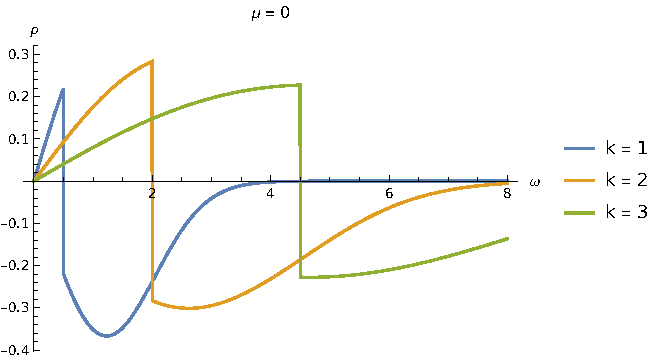
\includegraphics[width=.7\linewidth]{plots/spectralk.pdf}
	
	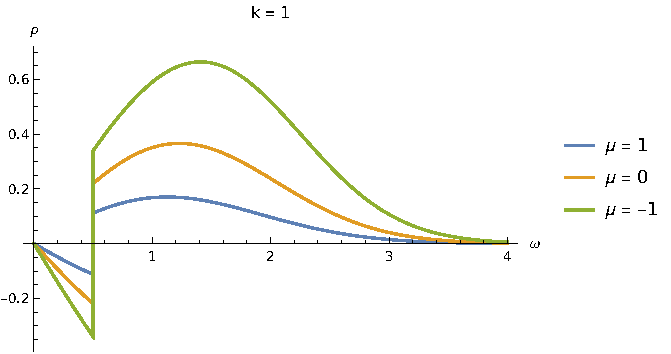
\includegraphics[width=.7\linewidth]{plots/spectralmu.pdf}
	\end{center}
	
	\newparagraph
	For the \textbf{spin correlations} $D_{ij}$, the above analysis still holds, and we need only change the source term in \eqref{eq:generating_functional} from $j(x)\,n(x)$ to $J^i(x)\,s_i(x)$. We have:
	\begin{equation}
	\begin{aligned}
		Z[j]
		&\sim \Bqty\Big{\,
				\det_{k,k',\bullet} \pqty{
					\beta D_0^{-1}(k)
						\,\delta_{k,k'}
					- \beta J_{k-k'}^i \sigma_i
				}
			}^{-1},\quad
		D_0^{-1}(k)
		= i\omega
			+ \tfrac{\vb{k}^2}{2m}
			- \mu \\
	\end{aligned}
	\end{equation}
	There are now no-trivial dependence on the spinor indices. After completing the trace of Pauli matrices, we find that the result is basically the same as before, but with an additional $\delta_{ij}$ factor:
	\begin{gather}
	\begin{aligned}
		W^{(2)}
		&= \frac{1}{2}
			\operatorname*{Tr}\limits_{k,k',\bullet}\,
			\sum_q
			\pqty\Big{
				J_{k-q}^i \sigma_i D_0(k)
			}
			\pqty\Big{
				J_{q-k'}^j \sigma_j D_0(q)
			} \\
		&= \frac{1}{2} \sum_q \sum_k
			J_{-q}^i
				\pqty\Big{
					\tr (\sigma_i\sigma_j)\,
					D_0(k)\,D_0(q + k)
				}
			J_{q}^j \\
		&= \frac{\beta V}{2} \sum_k
			J_{-k}^i D_{ij}(k)\, J_{k}^j,
	\end{aligned}
	\\
		D_{ij}(k)
		= \frac{1}{2} \tr (\sigma_i\sigma_j)
			D_n(k)
		= \delta_{ij} D_n(k),\quad
		\rho_{ij}
		= \delta_{ij} D_{ij}(k)
	\end{gather}
	This means that the spin correlation along a same direction is identical with the density correlation, while there is no correlation between spins in different directions. 
	
\printbibliography[%
%	title = {参考文献} %
	,heading = bibintoc
]
\end{document}
